\documentclass[compress]{beamer}
\usetheme{sthlm}

%-=-=-=-=-=-=-=-=-=-=-=-=-=-=-=-=-=-=-=-=-=-=-=-=
%        LOADING BEAMER PACKAGES
%-=-=-=-=-=-=-=-=-=-=-=-=-=-=-=-=-=-=-=-=-=-=-=-=

\usepackage{
booktabs,
datetime,
dtk-logos,
graphicx,
multicol,
pgfplots,
ragged2e,
tabularx,
tikz,
wasysym,
multirow,
float,
caption,
subcaption
}

\pgfplotsset{compat=1.8}

\usepackage[utf8]{inputenc}
\usepackage[portuguese]{babel}
\usepackage[T1]{fontenc}
\usepackage{newpxtext,newpxmath}
\usepackage{listings}

\lstset{ %
language=[LaTeX]TeX,
basicstyle=\normalsize\ttfamily,
keywordstyle=,
numbers=left,
numberstyle=\tiny\ttfamily,
stepnumber=1,
showspaces=false,
showstringspaces=false,
showtabs=false,
breaklines=true,
frame=tb,
framerule=0.5pt,
tabsize=4,
framexleftmargin=0.5em,
framexrightmargin=0.5em,
xleftmargin=0.5em,
xrightmargin=0.5em
}



%-=-=-=-=-=-=-=-=-=-=-=-=-=-=-=-=-=-=-=-=-=-=-=-=
%        LOADING TIKZ LIBRARIES
%-=-=-=-=-=-=-=-=-=-=-=-=-=-=-=-=-=-=-=-=-=-=-=-=

\usetikzlibrary{
backgrounds,
mindmap
}

%-=-=-=-=-=-=-=-=-=-=-=-=-=-=-=-=-=-=-=-=-=-=-=-=
%        BEAMER OPTIONS
%-=-=-=-=-=-=-=-=-=-=-=-=-=-=-=-=-=-=-=-=-=-=-=-=

\setbeameroption{show notes}

%-=-=-=-=-=-=-=-=-=-=-=-=-=-=-=-=-=-=-=-=-=-=-=-=
%        BEAMER COMMANDS
%-=-=-=-=-=-=-=-=-=-=-=-=-=-=-=-=-=-=-=-=-=-=-=-=


%-=-=-=-=-=-=-=-=-=-=-=-=-=-=-=-=-=-=-=-=-=-=-=-=
%
%	PRESENTATION INFORMATION
%
%-=-=-=-=-=-=-=-=-=-=-=-=-=-=-=-=-=-=-=-=-=-=-=-=

\title{Protocolos de \\ consistência}
\subtitle{DCE540 - Computação Paralela e Distribuída}
%\date{\small{\jobname}}
\author{\texttt{Iago Carvalho}}
\institute{\texttt{Departamento de Ciência da Computação}}

\hypersetup{
pdfauthor = {Iago A. Carvalho},      
pdfsubject = {Computação Paralela e Distribuída},
pdfkeywords = {},  
pdfmoddate= {D:\pdfdate},          
pdfcreator = {WriteLaTeX}
}

\begin{document}

\begin{frame}
\titlepage

\end{frame}

%% --------------------------------------------------------

\begin{frame}{Protocolo de consistência}

Define a real implementação do modelo de consistência
\begin{itemize}
    \item Como replicar
    \item Onde replicar
    \item Centrado no quê (ou em quem)?
    \begin{itemize}
        \item Nos dados
        \item Nos clientes
    \end{itemize}
\end{itemize}

\end{frame}

%% --------------------------------------------------------

\begin{frame}{Protocolos primários}

É a principal forma de implementação de consistência contínua
\begin{itemize}
    \item Também são protocolos de simples implementação
\end{itemize}

\vspace{0.5cm}

Existem dois protocolos básicos nesta classe
\begin{enumerate}
    \item Escrita remota (\textit{remote-write protocol})
    \item Escrita local (\textit{local-write protocol})
\end{enumerate}
\end{frame}

%% --------------------------------------------------------

\begin{frame}{Protocolo de escrita remota}

Neste protocolo o dado atualizado é centralizado
\begin{itemize}
    \item Existe um servidor de referência que sempre contém a versão mais atual de qualquer dado replicado
    \item O dado só pode ser alterado neste servidor principal
    \item Entretanto, existem replicações somente leitura em outros locais
\end{itemize}

\vspace{0.5cm}

Este protocolo é eficiente quando temos também um protocolo de invalidação
\begin{itemize}
    \item Ele marca as réplicas como desatualizadas
    \item Estas são atualizadas sob demanda
\end{itemize}

\vspace{0.5cm}

Este protocolo também é conhecido como \textit{primary-backup protocol}
\end{frame}

%% --------------------------------------------------------

\begin{frame}{Protocolo de escrita remota}

\centering 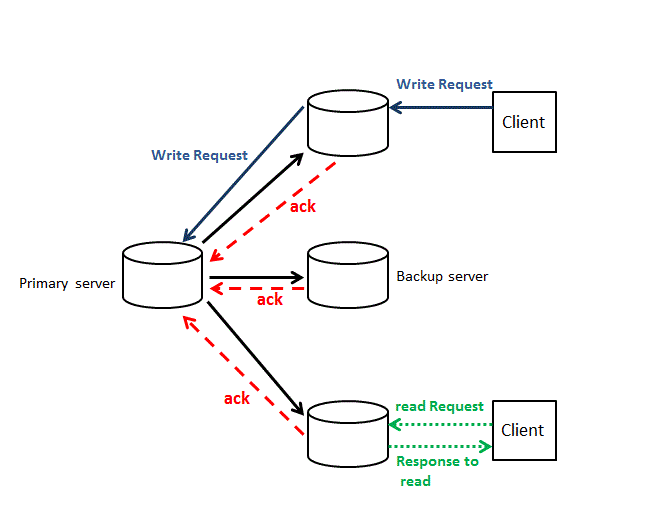
\includegraphics[width=0.93\textwidth]{images/remote-write.png}
\end{frame}

%% --------------------------------------------------------

\begin{frame}{Protocolo de escrita local}

Similar ao protocolo de escrita remota
\begin{itemize}
    \item Existe um único servidor que contém o dado atualizado
\end{itemize}

\vspace{0,5cm}

Entretanto, aqui o dado pode migrar de servidor para servidor
\begin{itemize}
    \item Onde o dado foi atualizado por último é considerado o novo servidor central
    \item Ajuda a tratar situações onde diversas atualizações em um conit são realizadas por um mesmo processo
\end{itemize}
\end{frame}

%% --------------------------------------------------------

\begin{frame}{Protocolo de escrita remota}

\centering 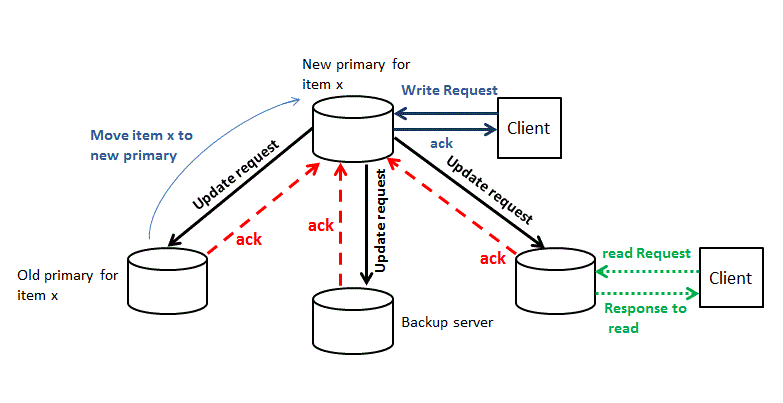
\includegraphics[width=0.93\textwidth]{images/local-write.png}
\end{frame}

%% --------------------------------------------------------

\begin{frame}{Replicação ativa}

Neste protocolo não existe um único dado considerado atualizado
\begin{itemize}
    \item Pelo contrário, é necessário atualizar todas as réplicas existentes
\end{itemize}

\vspace{0.5cm}

Quando um dado é atualizado, aquela operação de atualização é enviada a todas suas réplicas

\vspace{0.5cm}

Existe um problema de sincronização
\begin{itemize}
    \item Quando existem atualizações concorrentes, qual foi realizada primeiro?
    \begin{itemize}
        \item A solução é um esquema de \textit{multicast} totalmente ordenado
        \item Processo central coordenador (sequenciador)
    \end{itemize}
\end{itemize}
\end{frame}

%% --------------------------------------------------------

\begin{frame}{Atualização baseada em votos}

Neste protocolo, um cliente deve adquirir a permissão de acesso a múltiplas para que ele possa realizar operações de leitura ou escrita

\vspace{0.5cm}

Os votos são associados as permissões garantidas ao processo
\begin{itemize}
    \item Cada permissão concedida representa um voto
    \item Caso ele consiga permissões suficientes, pode então ler e escrever
    \item A operação de escrita gera um número de versão para o arquivo
\end{itemize}

\end{frame}

%% --------------------------------------------------------

\begin{frame}{Atualização baseada em votos}

Algumas regras devem ser seguidas para garantir um bom funcionamento do protocolo de atualização baseado em votos

\vspace{1cm}

\begin{minipage}{.55\textwidth}
\begin{itemize}
    \item $N \leftarrow$ Número de réplicas
    \item $N_R \leftarrow$ Quorum de leitura
    \item $N_W \leftarrow$ Quorum de escrita
\end{itemize}
\end{minipage}% <---------------- Note the use of "%"
\begin{minipage}{.44\textwidth}
$$
N_R + N_W > N
$$
$$
N_W > 0.5 N
$$
\end{minipage}

\end{frame}

%% --------------------------------------------------------

\begin{frame}{Protocolos de coerência de cache}

Estes protocolos não são muito diferentes dos anteriores

\vspace{0.5cm}

É necessário tratar 3 condições
\begin{enumerate}
    \item Quando as inconsistências são detectadas
    \item Como as réplicas de cache são mantidas nos servidores
    \item O que acontece quando um processo modifica um dado da cache
\end{enumerate}

\vspace{0.5cm}

Diversos protocolos podem ser construídos analisando variações destes 3 pontos

\end{frame}

%% --------------------------------------------------------

\begin{frame}{Protocolos de coerência de cache}

Estes protocolos não são muito diferentes dos anteriores

\vspace{0.5cm}

É necessário tratar 3 condições
\begin{enumerate}
    \item Quando as inconsistências são detectadas
    \item Como as réplicas de cache são mantidas nos servidores
    \item O que acontece quando um processo modifica um dado da cache
\end{enumerate}

\vspace{0.5cm}

Diversos protocolos podem ser construídos analisando variações destes 3 pontos

\end{frame}

%% --------------------------------------------------------

\begin{frame}{Consistência de dados centrados no cliente}

Para implementar consistência centrada no cliente, é necessário que cada operação de escrita possua um identificador
\begin{itemize}
    \item Indentificador global $W$
    \item Identificador é dado pelo servidor no qual a operação de escrita foi realizada
    \begin{itemize}
        \item Este servidor é denominado como servidor de origem de $W$
    \end{itemize}
\end{itemize}

\vspace{0.5cm}

Cada cliente guarda dois conjuntos de identificadores
\begin{enumerate}
    \item Relativos aos dados que ele realizou leitura
    \item Relativos aos dados que ele realizou escrita
\end{enumerate}
    
\end{frame}

%% --------------------------------------------------------

\begin{frame}{Leitura monotônica}

Durante uma operação de leitura, um cliente requisita o identificador do servidor
\begin{itemize}
    \item Identificador utilizado para verificar se sua cópia local está atualizada
    \item Caso não esteja atualizada
    \begin{itemize}
        \item Ele requisita a atualização do dado e realiza a leitura
    \end{itemize}
    \item Caso esteja atualizada
    \begin{itemize}
        \item Ele simplesmente realiza a leitura
    \end{itemize}
\end{itemize}
    
\end{frame}

%% --------------------------------------------------------

\begin{frame}{Escrita monotônica}

Similar a leitura monotônica

\vspace{0.5cm}

Durante uma operação de escrita, um cliente requisita o identificador do servidor
\begin{itemize}
    \item Identificador utilizado para verificar se sua cópia local está atualizada
    \item Caso não esteja atualizada
    \begin{itemize}
        \item Ele requisita a atualização do dado e realiza a leitura
    \end{itemize}
    \item Caso esteja atualizada
    \begin{itemize}
        \item Ele realiza a escrita
        \item Atualiza o identificador $W$
    \end{itemize}
\end{itemize}
    
\end{frame}

%% --------------------------------------------------------

\begin{frame}{Leia sua escrita}

O servidor onde a leitura está sendo realizada tem que ter ciência das escritas de todos os clientes
\begin{itemize}
    \item Ou seja, ele tem que ter a versão mais atualizada do dado
\end{itemize}
    
\vspace{0.5cm}

Isto gera uma grande sobrecarga na rede
\begin{itemize}
    \item Um servidor deve se comunicar com todos os outros
\end{itemize}

\end{frame}

%% --------------------------------------------------------

\begin{frame}{Escrita segue leitura}

Simplesmente necessita que o servidor verifique o identificador de todos os outros servidores

\vspace{0.5cm}

Caso ele possua o identificador mais atual, não faz nada

\vspace{0.5cm}

Caso ele possua um identificador ultrapassado, ele atualiza o dado
\begin{itemize}
    \item Assim, a escrita segue normalmente
    \item Os identificadores de leitura são atualizados
\end{itemize}

\end{frame}

\end{document}
